\documentclass{amsart}
\usepackage[margin=3cm]{geometry}                % See geometry.pdf to learn the layout options. There are lots.
\geometry{letterpaper}                   % ... or a4paper or a5paper or ...
%\geometry{landscape}                % Activate for for rotated page geometry
\usepackage[parfill]{parskip}    % Activate to begin paragraphs with an empty line rather than an indent
\usepackage{float}
\usepackage{graphicx}
\usepackage{amssymb}
\usepackage{epstopdf}
\usepackage{siunitx}
\usepackage{subcaption}

\DeclareGraphicsRule{.tif}{png}{.png}{`convert #1 `dirname #1`/`basename #1 .tif`.png}
\graphicspath{img/}

\title{Lab 9: Spectroscopy}
\author{Caspar \textsc{Lant}} % Author name

\date{\today} % Date for the report

\begin{document}

\bigskip

\maketitle % Insert the title, author and date
\begin{center}

Intermediate Experimental Physics I\\
\vspace{1.5cm}

\begin{tabular}{l r}

Section: & 002\\
\\
Date Performed: & December 2, 2015 \\ % Date the experiment was performed
Date Due: & December 9, 2015\\
\\
Partner: & Sam P. Meier \\ % Partner names
Professor: & Prof. Andrew Kent\\
Instructor: & David Mykytyn % Instructor/supervisor
\end{tabular}
\end{center}
\vspace{50mm}
\pagebreak

\paragraph{\textbf{The Objective} of this week's experiment was to put our vast theoretical knowledge of lenses to application. It is always a remarkable think to see what was once pure abstraction validated though rigorous scientific experimentation. }

\section{Theoretical Background/ Abstract}
\paragraph{Lenses have been of interest to us humans for a long time now. Convex lenses, concave lenses, even planar mirrors have all been the subjects of frenzied study through the ages. This should come as no surprise, given how fantastically useful they are to creatures who experience the world, mainly, through sight. We are mainly interested in what happens to the light from objects in front of the lens}
\begin{equation}
E = hv
\end{equation}
\begin{equation}
d\sin\theta = m\lambda (m = 0, \pm1, \pm2, \ ...)
\end{equation}
\begin{equation}
R = \dfrac{\lambda}{\Delta\lambda} = mN
\end{equation}

\subsection{The (PASCO) Grating Spectrometer}

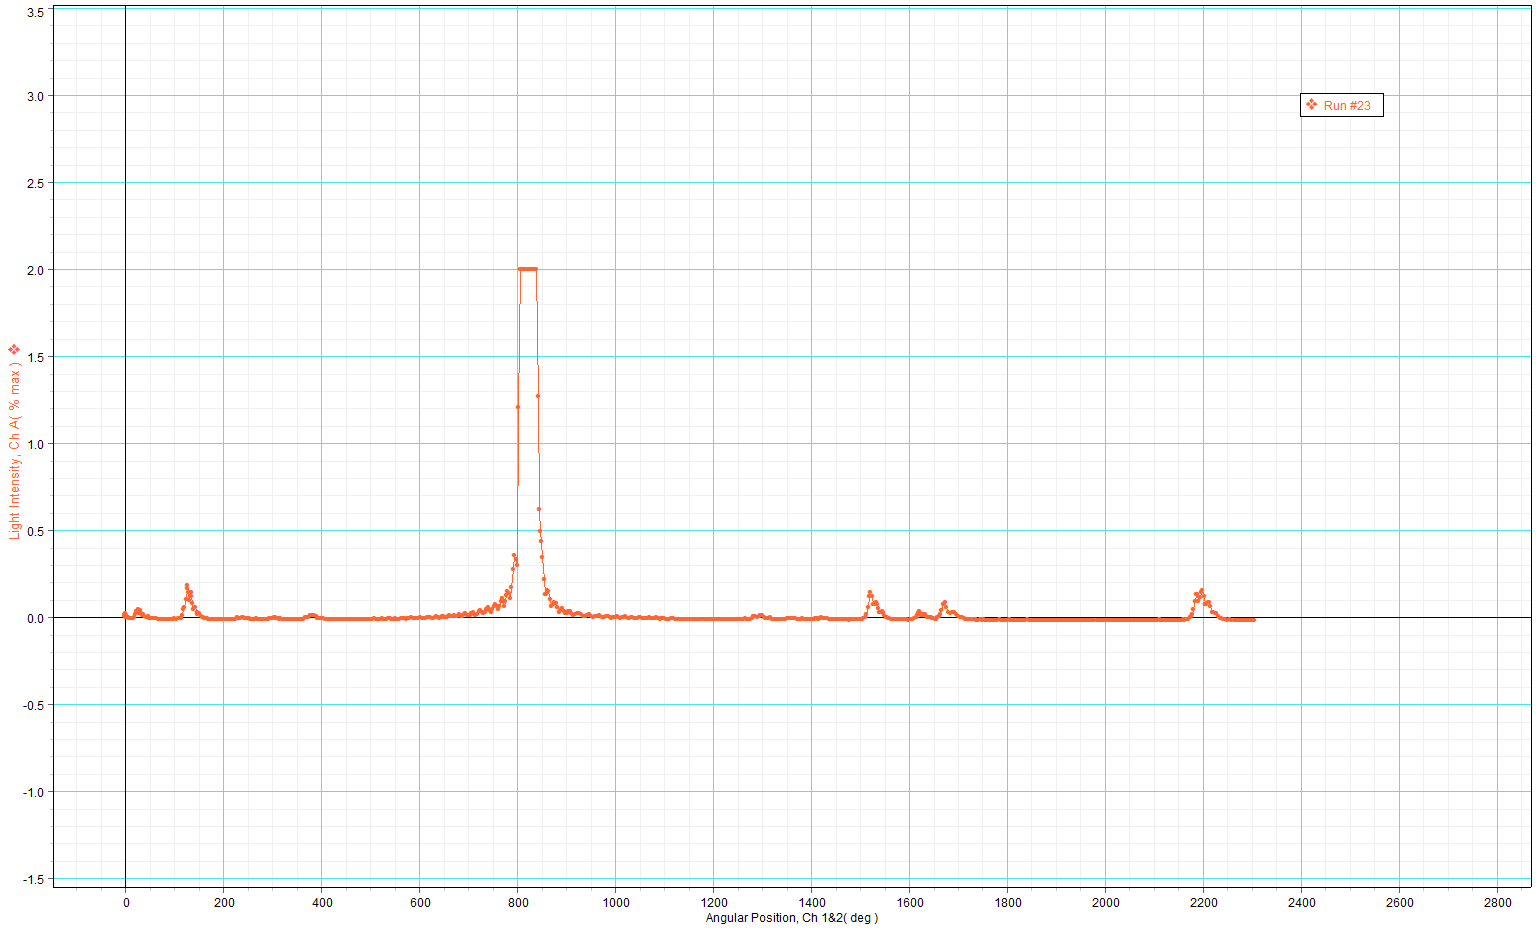
\includegraphics{he1.png}


\section{Experimental Procedure}
\begin{enumerate}
\item Begin by setting up the experiment as shown in the above diagram. You should make sure that all lenses and diffraction gradients are perpendicular the the axis of incoming light rays. 
\item Make doubly sure that the diffraction grating mounted to the protractor is oriented at zero degrees. 
\item Connect the rotary motion sensor and the light sensor to DataStudio, and set up the appropriate graphs and tables. 
\item Place the sodium lamp at the helm of the experimental boondoggle (apparatus)
\item It may help to place a slitted shade in the path of the sodium lamp to mitigate "leakage" of ambient light. This is a good place to tell you that you should be conducting your experiment in a darkened room.
\item Turn on the sodium lamp and focus the central maxima by changing the position of the image lens. 
\item Rotate the protractor such that the (faint) second-order line appears on the screen. 
\item Begin your experiment in DataStudio and rotate the the screen 
\item
\item
\item
\item
\item
\item
\end{enumerate}

\section{}

\medskip

\pagebreak

\section{Questions}

\begin{enumerate}
\item {\textit{What are appropriate units for $d$ and $\lambda$? For $\theta$?}
$d$ and $\lambda$ are both appropriately measured in units of length Nanometers seem to be on the right order of magnitude. Angles $\theta$ are, of course, measured in degrees or radians, but because we make the paraxial assumption $\theta\approx\sin\theta\approx\tan\theta$, it is also fine to treat these angles as dimensionless. 
\begin{quote}
Answer
\end{quote}}

\item{\textit{Calculate the wavelengths of lines X. Why do you not see them on the screen?}
\begin{quote}
Out of the frequency range for visible light
\end{quote}}

\end{enumerate}

\section{Error Analysis}




\end{document}
